%from
\subsection{Direct Wavefront Sensing}

In this sense, if in the focal region the specimen behaves as a point-like scatterer~(it will emit incoherent light) the sensor will be able to measure the aberrations produced in the emission path, which in principle they should be the same as in the illumination path.

But, if our specimen acts as a planar mirror-like in the focal region, the sensor will just be able to measure twice the even components of the aberrations produced in the illumination path~(or emission path), that is because the "`mirror behavior"' will spatially invert the aberrations in the illumination path~(Fig.~\ref{fig:abe_direct_sensing}). Let us analyze it in detail. We know that the measured aberration~($W(\rho,\phi)$) is the sum of the illumination an emission path aberrations. Also we can denote the measured aberration as the sum of its even and odd components. All together become,  

\begin{align}
	\ W(\rho,\phi) = {{W(\rho,\phi)_i}^{even}} + {{W(\rho,\phi)_i}^{odd}}+{{W(\rho,\phi)_e}^{even}} + {{W(\rho,\phi)_e}^{odd}},
	\label{eq:aberration_sum_il_em}
\end{align}  

Due to the spatial inversion we know that $W(\rho,\phi)_i^{even}=W(\rho,\phi)_e^{even}$ and $W(\rho,\phi)_e^{odd}=-W(\rho,\phi)_e^{odd}$, therefore the measured aberration can be simplified as,  

\begin{align}
	\ W(\rho,\phi)=2 {{W(\rho,\phi)_e}}
	\label{eq:ab_measured_spat_inver}
\end{align} 
 

\begin{figure}[htbp]
	\centering
		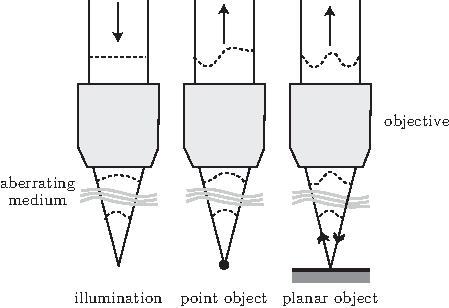
\includegraphics[width=0.50\textwidth]{images/abe_direct_sensing}
	\caption{Representation of the two effects due to the specimen structure on wavefront measurements. The left figure shows how the wavefront is aberrated in the illumination path. In the center it is shown a point-like scatterer. Only the emission path is measured. In the right figure it is shown a planar reflector. The illumination wavefront is spatially inverted on reflection before acquiring further aberration in the detection path. Image after~\cite{AOM_basic_ref}.}
	\label{fig:abe_direct_sensing}
\end{figure}


We have shown that in planar mirror-like structures we lose information about aberrations. Thus, in this cases it is not a good option to implement a direct sensing. Regarding microscopy techniques, we must note here that fluorescence emission is an incoherent process, but the non-linear processes generate a coherent signal.


%------------------------------------------------------------------------------
\subsubsection{Fluorescence Microscopy}
\label{sec:FlourescnecMicroscopy}

next section, all from \cite{wide_AOM_FM_spehrical_correction} uses a 
standard widefield flourescene microscope but use AOM to correct for 
spherical aberration due to depth -> no specimen induce correction
uses deconvolution to get out of foucs photons corrected

In this paper, we concentrate on the depth dependent aberration which can 
quickly become serious. Imaging 20 mum a live sample (index of refraction 1.36
) with an oil immersion lens causes the peak intensity of the point spread 
function (PSF) to drop 3-fold and the width of the PSF in the axial direction 
to increase by 2-folds. \cite{wide_AOM_FM_spehrical_correction} 

Because wide-field microscopy captures as efficiently as possible every 
emitted photon ultimately minimizing the sample excitation dose, it is well 
suited to in vivo imaging in samples where scattering is not too large. 
Although the out-of-focus photons are in the wrong place, they can be 
effectively re-assigned to the location of emission by constrained 
deconvolution algorithms \cite{wide_deconvolution}

The problem of depth aberrations can be solved by matching the sample index 
and the index of the immersion medium, but this is frequently not feasible or 
desirable. For example, the index of fixed cells can be matched to that of 
the immersion oil, but this option is not available for live imaging.

An important drawback to most schemes that have been proposed so far is that 
they require several images to be taken to optimize the aberration 
correction. This presents a serious problem for live imaging in biology 
because the fluorescence intensities can be weak and susceptible to rapid 
bleaching.

The approach we follow is to correct the depth aberrations withanopen-loop 
predictive algorithm similar totheapproach taken by Potsaid et al. in 
correcting off-axis aberrations. This is possible because the depth 
aberration can be calculated for a given depth into the sample. The depth 
aberration is the result of depth-dependent path length differences.

Correcting depth aberrations with a DM improves both the peak intensities and 
the deconvolution of images taken below the cover slip by removing the depth 
aberration. This allows the use of fast space-invariant deconvolution 
algorithms instead of depth-dependent algorithms. This is significant because 
it improves both the signal-to-noise ratio and the resolution in biological 
imaging where photons are in short supply. Unfortunately, the performance 
does not yet achieve what is theoretically possible.

\begin{figure}[htb]
	\centering
		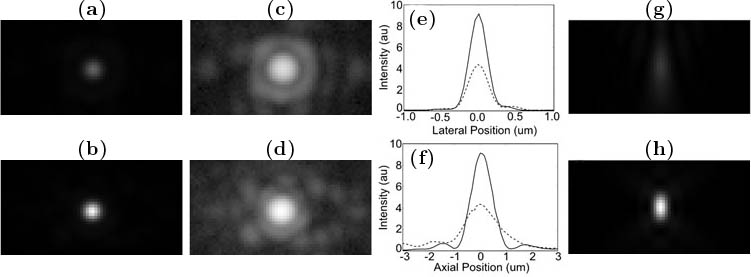
\includegraphics[width=0.80\textwidth]{images/wide_flour_spher_All.jpg}
	\caption{Images of a $\unit[200]{nm}$ bead $\unit[67]{\upmu m}$ below the 
cover slip in a water/glycerol mixture with n = 1.42.  (a) Uncorrected image 
of in-focus plane. (b) Corrected image of in-focus plane. Images (c) and (d) 
are the same as (a) and (b), respectively, but on a logarithmic scale for 
better visualization. (e) and (f) are line profiles of the intensity through 
the center of the bead along the lateral and the longitudinal axis, 
respectively. The dashed line is from the uncorrected image and the solid 
line is from the corrected image. (g) and (h) are simulations of the PSF. 
Images based on \cite{wide_AOM_FM_spehrical_correction}.}
	\label{fig:wide_flour_spher_All} 
\end{figure}


The first is the effect of uncorrected aberrations from the sample and the 
optical path, which decrease the maximum intensity at the cover slip, but in 
a way that does not add linearly to the depth aberration. Thus only a 
fraction of the dispersed photons can be restored to the central peak. In 
closed loop AO systems, system aberrations are automatically compensated at 
each position (Wright et al., 2007), but in an open-loop system this is not 
possible. The second factor is the inability of the mirror to precisely 
conform to the shape given by Eq. (1). The residual error of the mirror shape 
increases with depth (see Fig. 3c) so that as the imaging plane goes deeper 
and the possibility for improvement becomes greater, the improvement in peak 
intensities decreases

Lastly, the ultimate goal of applying adaptive optics in microscopy is to 
correct all aberrations including those introduced by the refractive index 
variations of the sample itself.
\cite{wide_AOM_FM_spehrical_correction}


\begin{figure}
	\centering
		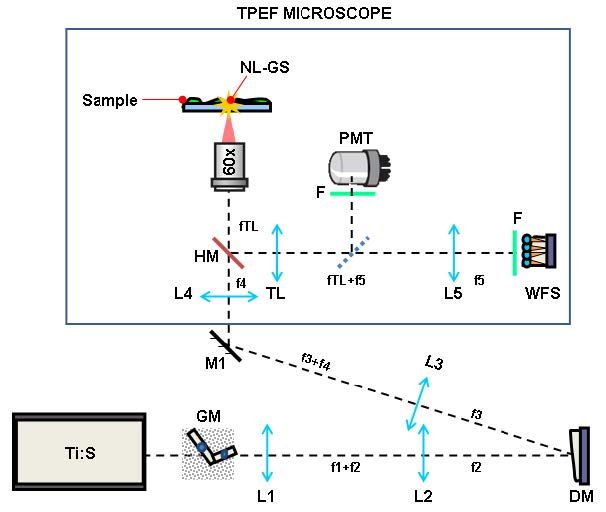
\includegraphics[width=0.75\textwidth]{images/TPFM_guide-star}
	\caption{Experimental setup for aberration corrected two-photon fluorescence microscopy as proposed by \emph{Aviles-Espinosa et al.}. GM - galvanometric mirrors, L1-L5 - lenses, DM - deformable mirror, M1 - mirror, HM - filter and beamsplitter, MO - microscope objective, TL - microscope tube lens, F - band pass filters, PMT - photo multiplier tube, WFS - Shack-Hartmann wavefront sensor. The microscope output port is manually selected either for the PMT or for the WF sensor using PS. See~\cite{scan_TPFM_guide_start} for the original image as well as a detailed description of the working principle.}
	\label{fig:TPFM_guide-star}
\end{figure}
%
probably drop all this...
Before the authors started their experiments on biological samples, they first showed that the guide star is reproducible, reliable and independent from the excitation beam aberrations. They continued to verify that the NL-GS behaves as point source as well as proving that aberrations are similar in the complete Field Of View (FOV). Since all these requirements were met, it was show that aberrations in the imaged area can be effectively corrected using only one NL-GS. The authors then continued to calibrate their system, eliminating the passive aberrations of the microscope system coming from the optics for excitation beam as well as the beam path from the objective pupil to the output ports of the microscope. These so called coupling aberrations only need to be corrected once for a given microscopic setup. They were measured and taken into account as a reference for all the subsequent wavefront measurements. The second correction step was to measure the so called focusing aberrations caused by the focusing part of the system. This step was performed every time prior to the actual image acquisition to account for the specific measurement~(i.e. the objective, the refractive index matching oil, the cover slip and the sample).\newline

The aberrations can also change significantly with depth and hence using the same correction for different depths can result in a degradation of the image quality.  The correction can however be adapted for different imaging depths in the sample. This permits improvement of the image quality throughout an axially extended sample. It is furthermore possible to determined the appropriate modes once and use the same scheme for any specimen, as the scheme is mostly independent of the object structure. Alternatively, if one wants to correct for local variations in aberrations the image could be formed from several sub-images for which independent aberration correction would be performed.